\section{原型系统设计与实现}
本章将根据前文对基于P2P网络的信息自主流动机制的讨论,设计并实现一套较为完善的原型系统。这里系统是指运行在每个节点上既能充当服务器发送信息、也能充当客户端接受信息,我们称之为节点系统。本章将分别从节点系统架构、数据库、功能模块等方面入手,详细讨论各个实现环节的细节,最后将展示简单的客户端截图。

\subsection{主要开发技术}
节点系统主要用Java编程语言实现,辅以Python作为数据分析之用,模块间与系统间的消息传递格式为JSON,具体技术如表\ref{tbl:tech}。鉴于本系统只是一个雏形,因此使用了大量轻量级框架进行敏捷开发,在并发性等性能方面的问题暂时先不纳入考虑。

\begin{table}[ht]
\centering
\caption{原型系统开发主要技术列表}
\begin{tabular}{|c|c|} 
\hline
操作系统:& OS X 10.10.3 \\
\hline
系统后台开发语言:& JDK 1.8 \\
\hline
系统后台开发框架:& JFinal\footnote{http://www.jfinal.com/} \\
\hline
后台数据库:& sqlite 3 \\
\hline
系统前端开发语言:& Html、CSS、Javascript \\
\hline
系统前端开发框架:& Bootstrap、JQuery \\
\hline
数据引擎开发语言:& Python 2.7、R \\
\hline
数据引擎计算框架:& numpy、scipy、sklearn、gensim、NLTK \\
\hline
\end{tabular}
\label{tbl:tech}
\end{table}

\subsection{节点系统的架构设计}
首先,节点系统的最大特点是既要充当服务器向外部的节点进行交互信息,也要作为客户端为本地用户提供一个可视化的浏览平台。为了满足这样的需求,节点系统的架构设计如图\ref{fig:architect}所示。

\begin{figure}[!ht]
\centering
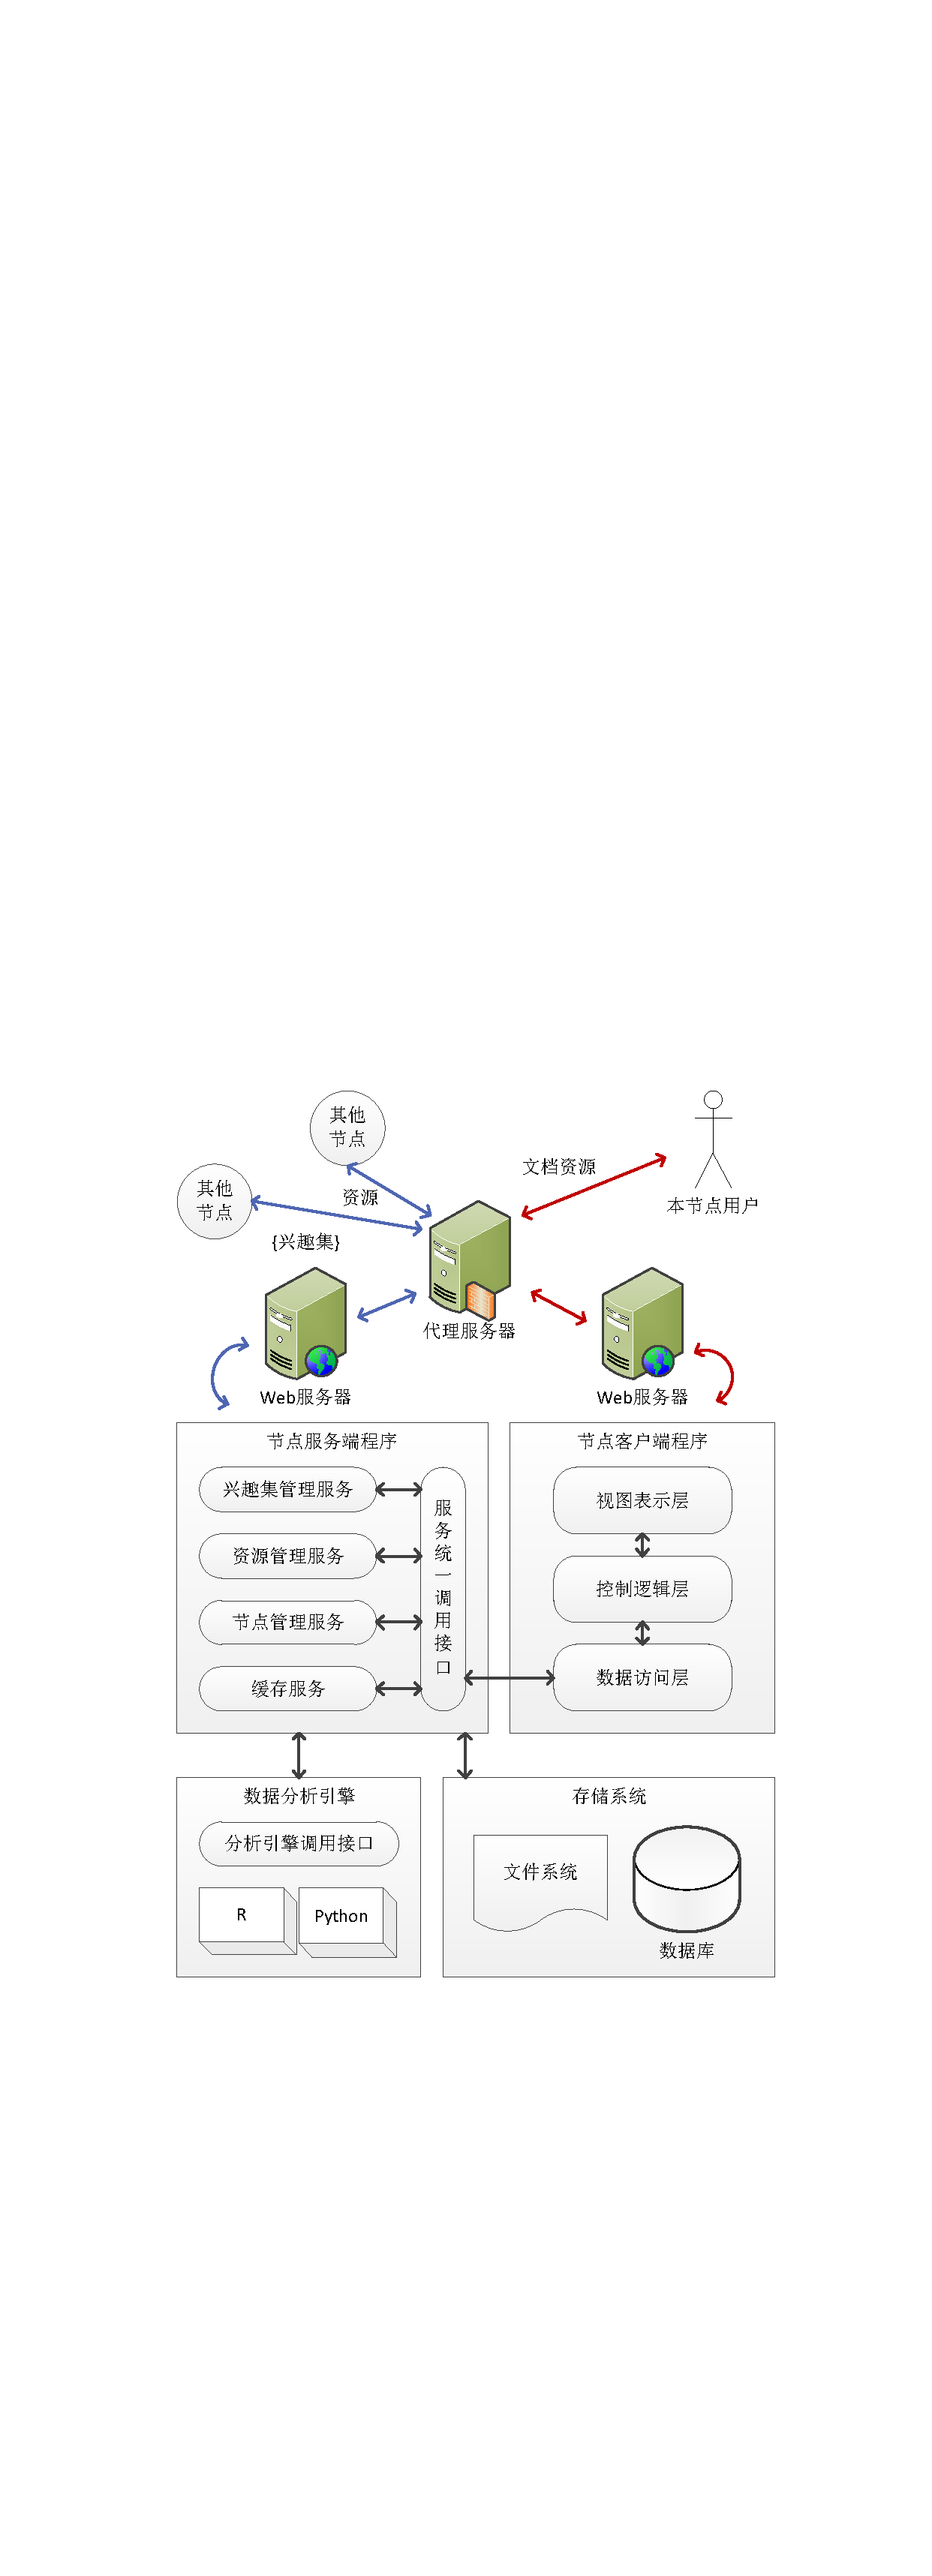
\includegraphics[width=\textwidth]{architect.pdf}
\caption{节点系统的架构示意图}
\label{fig:architect}
\end{figure}

从图中可以看到,节点系统处理的请求用户可以分为两大类:本节点的用户和其他节点的程序。其中,本节点的用户主要是对本地资源进行操作,包括发表新的文章、查看推荐的文章等。而其他节点的程序主要是与本节点交换兴趣信息和网络信息等。考虑到两种请求的独立性,我们将节点系统分为节点服务端程序和节点客户端程序两大模块,并分别运行于两个独立的web服务器中,并由代理服务器统一接受、处理并转发双方的请求。这样做的好处是模块之间保持相对地独立,作用分工明确,耦合性也比较小。

对于节点客户端程序,本质是一个运行在web服务器上的网站系统,由于其功能相对简单,主要是对资源数据的读写,因此在架构设计方面采用了如下两点方案:
\begin{itemize}
  \item 纯MVC架构:在传统的J2EE架构中,控制层和业务逻辑层往往是分开的
  \item 切断数据访问:
\end{itemize}

\subsection{节点系统的数据库设计}

\subsection{节点系统的功能设计}

\subsection{节点系统的界面展示}

\subsection{小结}
